\chapter{Auswirkungen von unterschiedlichen Kameraauflösungen}
\label{sec:minimalAuf} 


Aufbauend auf dem entstandenen Szenenrekonstruktionsalgorithmus für Kameras mit gleicher Auflösung, wurde der Algorithmus dhingehend getestet, ob eine Szenenrekonstruktion auch möglich ist, wenn gilt, dass $\zeta \neq \zeta'$. Zunächst wird beschrieben, was genau bei der Umstellung der Auflösung auf einem Sensor sich verändert. Anschließend wird analysiert, wie sich die Auflösungsänderung auf das in Kapitel \ref{sec:CameraModels} beschriebene Kameramodell ändert und welche Einflüsse sie auf die in Kapitel \ref{sec:HFE} hergeleiteten Epipolaren Bedingungen hat. Zum Schluss werden die Ergebnisse des synthetischen Beispiels mit unterschiedlichen Kameraauflösungen präsentiert und validiert.
 
%Igendwie sagen, dass wie gezeigt wurde der Ansatz für gleiche Auflösungen funktioniert hat. sRoll im folgendenden die möglichkeit in betracht gezogen werden dass $\zeta \neq \zeta'$. Dazu soll erst einmal erklärt werden, was es für den Sensor bedeutet, wenn sich eine Auflösung ändert und was es bedeutet wenn sich zusätzlich auch noch die Seitenverhältnisse ändern.
%%Im vorherigen Kapitel wurde gezeigt, wie eine 3D-Szene aus zwei heterogenen Bildquellen, welche von zwei Kameras gleicher Auflösung aufgenommen wurden, rekonstruiert wurden und gleichzeitig noch die externen Kameraparameter von $C'$ in Relation zu $C$ geschätzt wurden.
%
%
%Dies wirft die Frage auf, welche Auswirkungen Bilder zweier Kameras mit unterschiedlichen Auflösungen auf die Funktionen den Szenenrekonstruktionsalgorithmus haben. 
%
%
%Was genau unterschiedliche Auflösungen der Kameras für die einzelnen Bilder bedeutet und was genau sich bei der Aufnahme mit dem Sensor dabei ändert, soll im folgenden Unterkapitel kurz erläutert werden. 
%
%Danach soll analysiert werden, ob eine veränderte Bildauflösung Auswirkungen auf die in Kapitel \ref{sec:HFE} hergeleiteten Abildungsvorschriften hat. Als letztes wird im synthetischen Beispiel die Auflösung einer Kamera mehrmals verändert und der Szenenrekonstruktionsalgorithmus angewandt. Das Ergebnis des Algorithmus wird analysiert und validiert. 

%Danach wird aufgezeigt, was genau diese Veränderungen für die in Kapitel \ref{sec:HFE} Hergeleiteten Bedingungen Epipolargeometrie bedeuten und letztendlich wird das Minimalbeispiel so angepasst, als hätten zwei Kameras unterschiedlicher Auflösung die selbe Szene wie davor aufgenommen und die Resultate miteinander verglichen. 

\section{Geometrie eines Sensors}


Die Geometrie eines Sensors kann als eine  $M \times N$ - Matrix, bestehend aus $M \times N$ Sensorelementen dargestellt werden\cite{Photonik}. Die Auflösung eines Sensors hängt von den horizontalen und vertikalen Abständen der Sensorelemente ab. Abbildung \ref{fig:Sensor} zeigt den schematischen Aufbau eines Sensors (CMOS). 

\begin{minipage}{\linewidth}
	\centering
	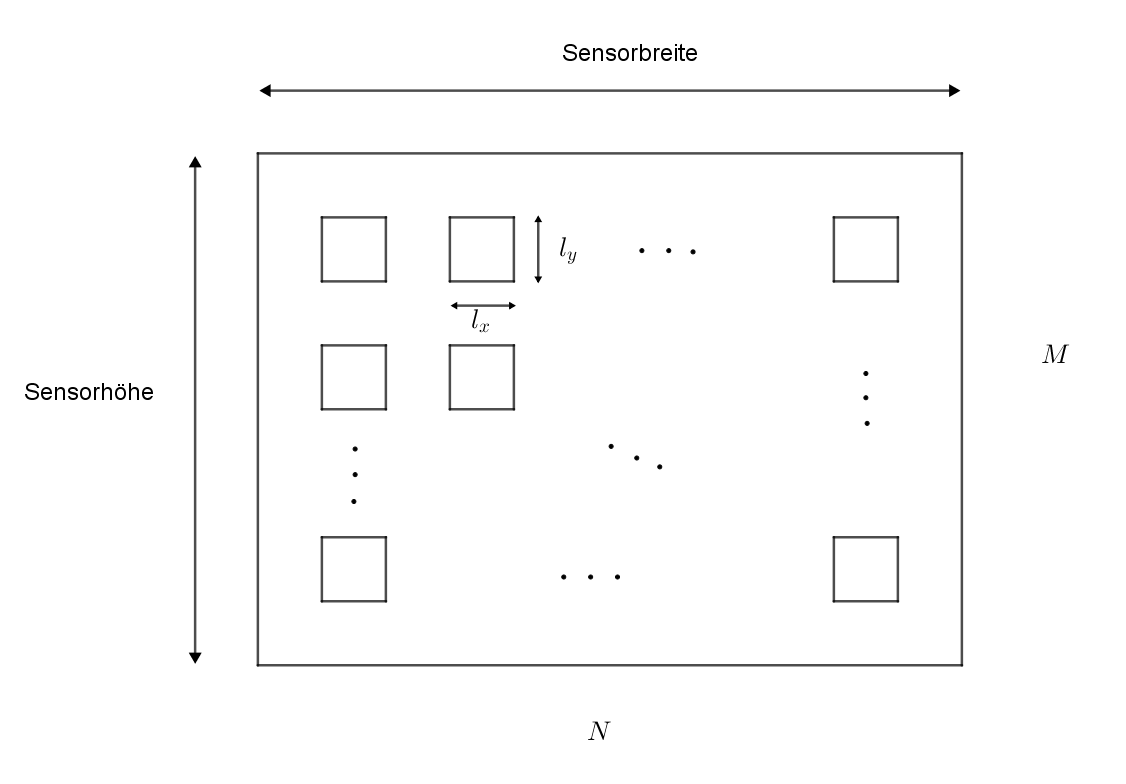
\includegraphics[width=.8\linewidth]{images/Bildsensor_mit_Pixel.png}
	\captionof{figure}{Rechteckiger Bildsensor mit darauf sich befindendenden quadratischen Sensorelementen. Vergleiche \cite{Photonik}} 
	\label{fig:Sensor}
\end{minipage}\\ \\


Ein Sensor hat eine maximale Auflösung. Bei maximaler Auflösung definiert genau ein Sensorelement einen Pixel. Ein Pixel wiederum entspricht einem Bildpunkt\cite{Photonik}. Die Bildqualität ist abhängig von der Größe des Sensorchips und der Menge der sich darauf befindenden Sensorelemente. Wird eine Auflösung kleiner der maximal möglichen Auflösung eingestellt, desto geringer wird die Anzahl der Pixel. Der Prozess, welcher hier stattfindet, gehört zu den Nachbarschaftsoperationen\cite{Photonik}. Ein neuer Pixel wird aus den benachbarten Pixeln berechnet. Dabei nehmen alle Pixel, die sich zum neuen Pixel zusammengeschlossen haben, die gleichen Farbwerte an. \\

Eine Veränderung der Auflösung auch eine Änderung der Seitenverhältnisse mit einschließen. Ändert sich das Seitenverhältnis so wird der Bereich der lichtempfindlichen Fläche auf dem Sensor beschränkt\cite{Photonik}. Abbildung \ref{fig:SensorResolutions} stellt schematisch da wie sich die lichtempfindlichen Bereiche auf dem Sensor bei unterschiedlichen Auflösungen ändert.


\begin{minipage}{\linewidth}
	\centering
	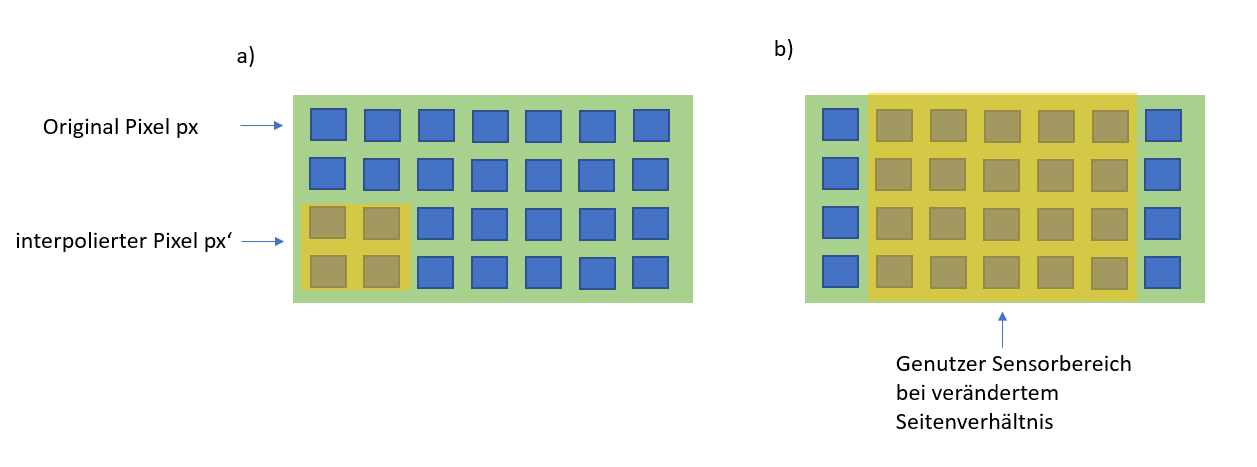
\includegraphics[width=1.\linewidth]{images/AufloesungSensor.png}
	\captionof{figure}{Bild a) zeigt die den Zusammenschluss mehrerer benachbarter Pixel zu einem neuen Pixel. Bild b) zeigt in gelb markiert, den aktiven lichtempfindlichen Bereich des Sensors, wenn sich das Seitenverhältnis geändert wird und nicht mehr der komplette Sensor genutzt wird.} 
	\label{fig:SensorResolutions}
\end{minipage}\\ \\

\section{Auswirkungen auf die Szenenrekonstruktion}

Im folgenden soll analysiert werden, welche Änderungen sich im Lochkameramodell bei veränderte Auflösung ergeben und was für Auswirkungen diese auf den,  \textit{Epipolar-Constraints} haben, gerade in Bezug auf die Bestimmung der extrinsischen Kameraparameter.\\

Im Lochkameramodell verändert sich mit ändernder Auflösung der Kamera lediglicht die Skalierung der Sensorkoordinatenachsen. Diese orientieren sich wie in Kapitel \ref{sec:CameraModels} beschrieben an längenskalierung der Pixelkanten $l_x$ und $l_y$. Wird die Auflösung einer Kamera verändert, so ändern sich die Anzahl und die Größe der Pixel. Folglich kommt es zu einer Skalierung des Sensorkoordinatensystems.Für alle anderen Koordinatensysteme ändert sich nichts. Während sich für dein Punkt im Sensorkoordinatensystem neue skalierte Koordinaten ergeben, so bleibt der Bildpunkt in Bildebenenkoordinaten unverändert. Durch Nachbarschaftsopterationen werden aus mehreren benachbarten Pixel ein neuer, jedoch bleibt der Ort des Pixel der gleiche\cite{Doessel}.
Die Abbildungen \ref{fig:Aufl1} und \ref{fig:Aufl2} zeigen, dass sich zwar das Mapping von Bildebenenkoordinatensystem auf das Sensorsystem ändert, Jedoch wird der Bildpunkt $m_{\tau'}$ an der selben Position des Sensors wie zuvor auch abgebildet.\\


\begin{figure}[!htb]
	\minipage{0.48\textwidth}
	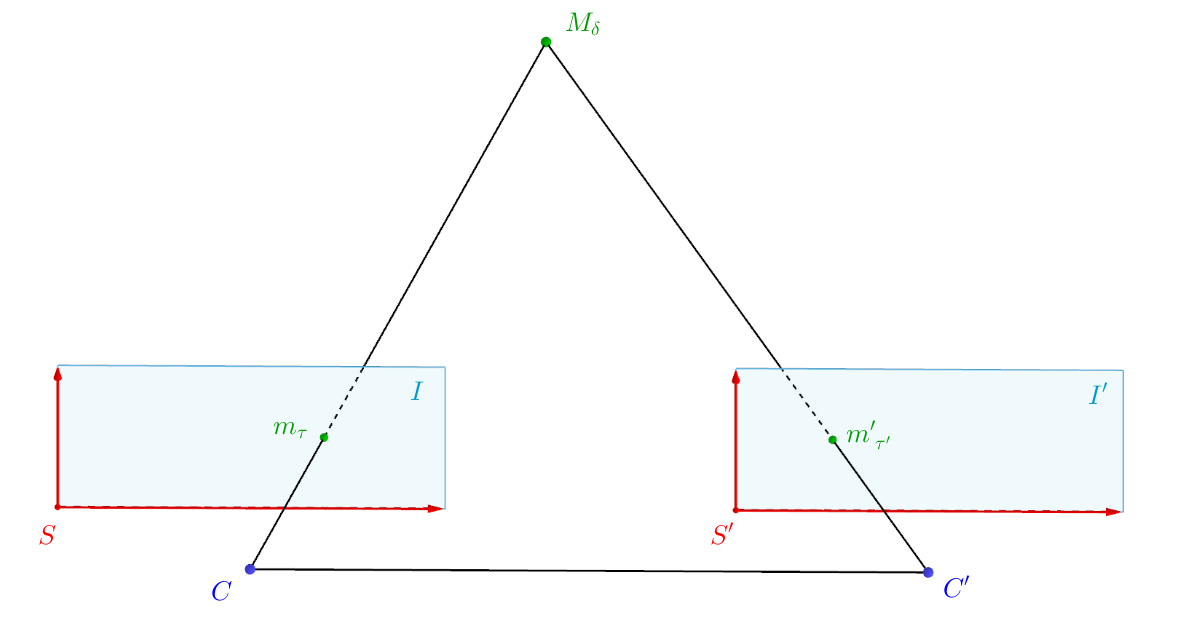
\includegraphics[width=\linewidth]{images/SensorSelbeAufloesung_beschriftet.png}
	\caption{$C$ und $C'$ haben die selbe Auflösung eingestellt}
	\label{fig:Aufl1}
	\endminipage\hfill
	\minipage{0.49\textwidth}
	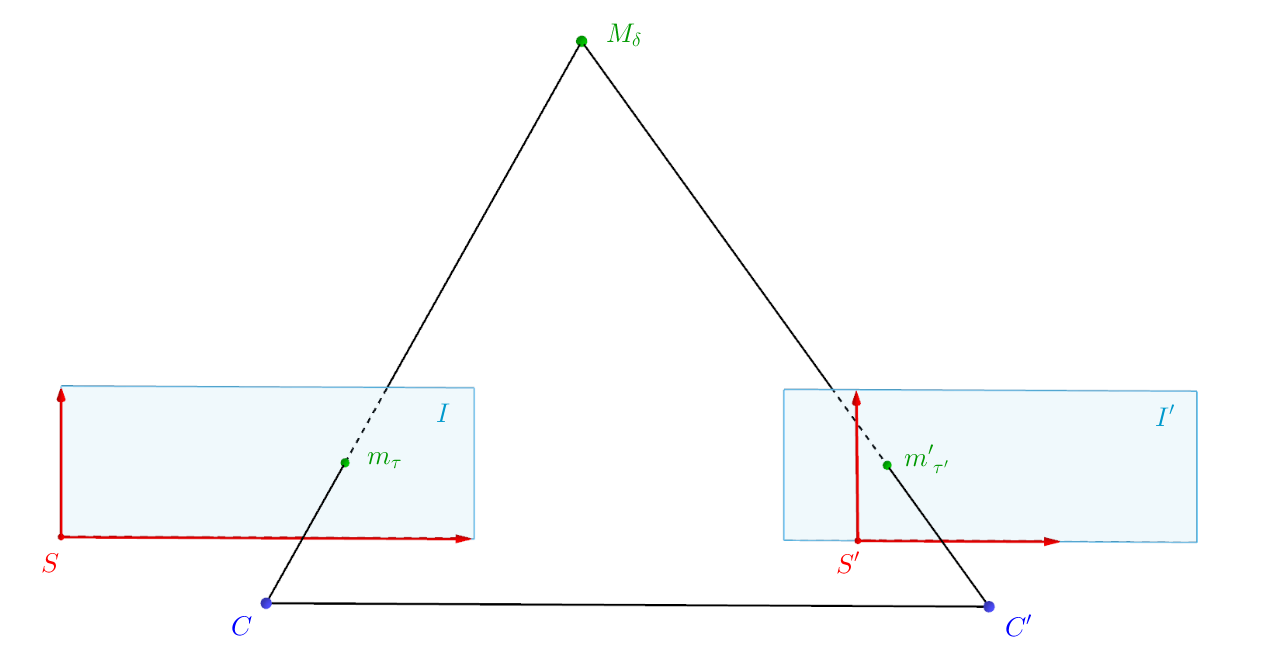
\includegraphics[width=\linewidth]{images/SensorUnterschiedlicheAufloesung_beschriftet.png}
	\caption{$C$ und $C'$ haben unterschiedliche Auflösungen eingestellt}
	\label{fig:Aufl2}
	\endminipage\hfill
\end{figure}


Eine Skalierung der Sensorkoordinaten führt eine Skalierung der Kameramatrix mit sich. Wie in Kapitel \ref{sec:CameraModels} gezeigt, setzt sich die erweiterte Kameramatrix $K$ wie folgt zusammen:

\begin{equation}
K=	R_\sigma K_0=  \begin{bmatrix}
k_x \zeta & 0 & V_{\sigma,x}\\
0 & k_y \zeta & V_{\sigma,y}\\
0 & 0   & 1 &\\
\end{bmatrix}
\end{equation}

Wird die Kameraauflösung verändert so bleibt die Brennweite $\zeta_x$ und $\zeta_y$ effektiv die gleiche, da sich aber die skalierung der Pixel mit $k_x$ und $k_y$ ändert, ist die Brennweite in Pixeln ausgedrückt verändert. Im synthetischen Beispiel wurde die Auflösung von $K'$ verändert indem, die Werte $\zeta'_x$ und $\zeta'_y$ durch multiplikation mit einem Salierungsfaktor verändert wurden.\\

Um die Aufgestellte Theorie zu überprüfen, wurde im synthetischen Beispiel die Kameramatrix von einer der beiden Kameras modifiziert. Für $C$ wurde $\zeta_x = \zeta_y = 1$ definiert, so das für Kameramatrix $K$ gilt:

\begin{gather}
	K = \begin{bmatrix}
		1&0&0&0\\
		0&1&0&0\\
		0&0&1&0\\
		%0&0&1&0
	\end{bmatrix}
\end{gather}


Die Kamermatrix $K'$ von $C'$ galt ursprünglich, dass $K = K'$. Die Auflösung von $C'$ wird geändert indem ein Skalierungsfaktor mit $\zeta'_x$ und $\zeta_y$ multipliziert wird. Für das Beispiel wurden drei verschiedenen Auflösungen getestet.  $K'_1$ mit $\zeta'_x \cdot 2$ und $\zeta'_y \cdot 2$, $K'_2$ mit $\zeta'_x \cdot 3.2$ und $\zeta'_y \cdot 1.2$ und $K'_e$ mit $\zeta'_x \cdot 0.5$ und $\zeta'_y \cdot 4.3$. Da ursprünglich galt, dass $\zeta'_x =\zeta'_y = 1$ ergeben sich die folgenden Kameramatrizen für $K'$.
%Während für die Kameramatrix von $C$ der Wert  $\zeta_x = \zeta_y = 1$ ist, wird in der Kamermatrix $K$ ist, wird das $\zeta$ in $C'$ verändert, so dass drei verschiedene neue Kameramatrizen $K'_1, K'_2$ und $K'_3$ ergeben. 



\begin{gather}
	K'_1 = \begin{bmatrix}
		2&0&0&0\\
		0&2&0&0\\
		0&0&1&0\\
		%0&0&1&0
	\end{bmatrix}\\
	K'_2 = \begin{bmatrix}
		3.2&0&0&0\\
		0&1.2&0&0\\
		0&0&1&0\\
		%0&0&1&0
	\end{bmatrix}\\
	K'_3 = \begin{bmatrix}
		0.5&0&0&0\\
		0&4.3&0&0\\
		0&0&1&0\\
		%0&0&1&0
	\end{bmatrix}
\end{gather}\\

Die Unterschiede der enstehenden Abbildungen in $C'$ sind in den Abbildungen \ref{fig:K}, \ref{fig:K1},\ref{fig:K2} und \ref{fig:K3} zu sehen. \\
 
 
\begin{figure}[!htb]
	\minipage{0.48\textwidth}
	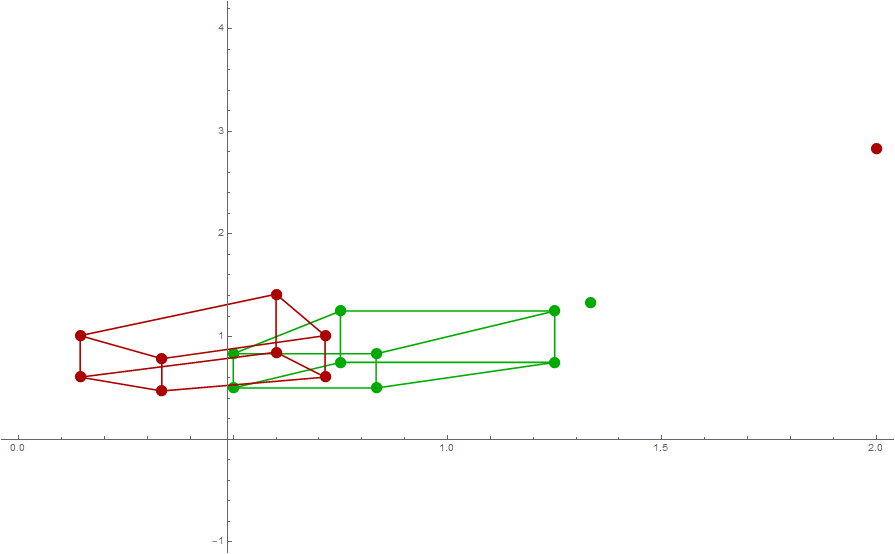
\includegraphics[width=\linewidth]{images/Zeta1.png}
	\caption{$C$ und $C'$ haben die selbe Auflösung eingestellt}
	\label{fig:K}
	\endminipage\hfill
	\minipage{0.48\textwidth}
	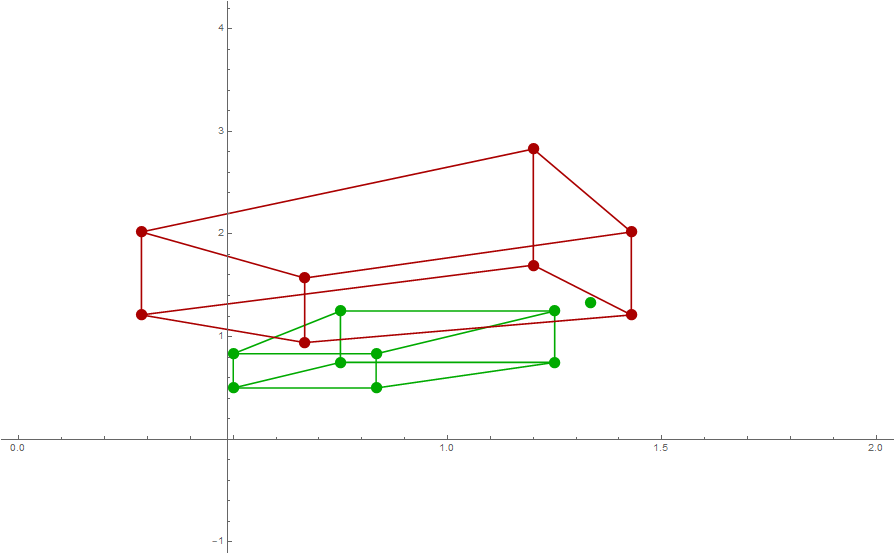
\includegraphics[width=\linewidth]{images/Zeta2.png}
	\caption{$C$ und $C'$ haben unterschiedliche Auflösungen eingestellt. $C$ mit $K$ und $C'$ mit $K_1'$}
	\label{fig:K1}
	\endminipage\hfill
\end{figure}

\begin{figure}[!htb]
	\minipage{0.48\textwidth}
	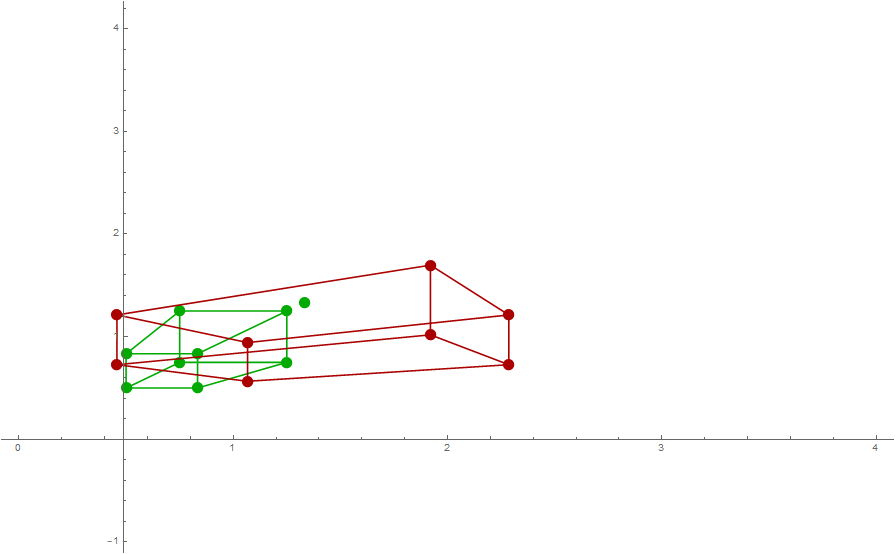
\includegraphics[width=\linewidth]{images/Zeta32_12.png}
	\caption{$C$ mit $K$ und $C'$ mit $K_2'$}
	\label{fig:K2}
	\endminipage\hfill
	\minipage{0.48\textwidth}
	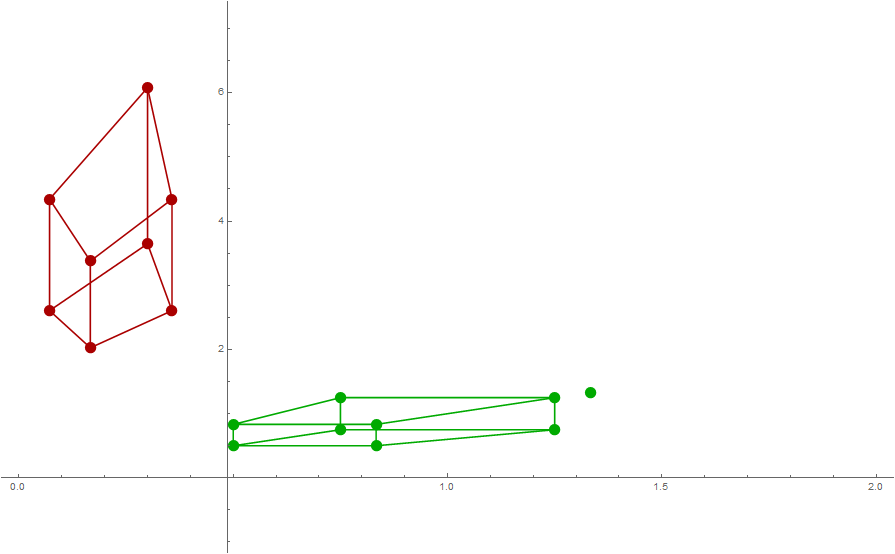
\includegraphics[width=\linewidth]{images/Zeta05_43.png}
	\caption{$C$ mit $K$ und $C'$ mit $K_3'$}
	\label{fig:K3}
	\endminipage\hfill
\end{figure}
\pagebreak

Wird das synthetische Beispiel jeweils mit den drei verschiedenen modifizierten $K'$ durchgerechnet, so ergeben sich für die essentielle Matrix folgende Ergebnisse.

\begin{gather*}
	\zeta'_x = 1, \, \zeta'_y = 1: \; \; \;\;
	E = \begin{pmatrix}
		0&-0.5&0\\
		0&0&\frac{1}{\sqrt{2}}\\
		0&0.5&0
	\end{pmatrix} |: 0.5 \; \leadsto
	E = \begin{pmatrix}
		0&-1&0\\
		0&0&-\sqrt{2}\\
		0&1&0
	\end{pmatrix}\\
	\zeta'_x = 2, \, \zeta'_y = 2: \; \; \;\;
	E = \begin{pmatrix}
		0&0.756&0\\
		0&0&1.069\\
		0&-0.756&0
	\end{pmatrix} |: -0.756 \; \leadsto
	E = \begin{pmatrix}
		0&-1&0\\
		0&0&-\sqrt{2}\\
		0&1&0
	\end{pmatrix}\\
	\zeta'_x = 3.2, \, \zeta'_y = 1.2: \; \; \;\;
	E = \begin{pmatrix}
		0&0.634&0\\
		0&0&1.069\\
		0&-0.634&0
	\end{pmatrix} |: -0.634 \; \leadsto
	E = \begin{pmatrix}
		0&-1&0\\
		0&0&-\sqrt{2}\\
		0&1&0
	\end{pmatrix}\\
	\zeta'_x = 0.5, \, \zeta'_y = 4.3: \; \; \;\;
	E = \begin{pmatrix}
		0&0.442&0\\
		0&0&1.069\\
		0&-0.442&0
	\end{pmatrix} |: -0.442 \; \leadsto
	E = \begin{pmatrix}
		0&-1&0\\
		0&0&-\sqrt{2}\\
		0&1&0
	\end{pmatrix}\\
\end{gather*}

Wie beobachtet werden kann, werden, trotz unterschiedlicher Kameraauflösungen für $K'$, immer die selbe essentielle Matrix im algorithmus bestimmt. Dies lässt sich mit Hilfe des \textit{Epipolar-Constraints} von $E$ aus Gleichung \ref{eq:Ep7} genauer erläutern.\\


Die Fundamentalmatrix beinhaltet, sowohl die intrinsischen als auch die extrinsischen Parameter, um von $F$ auf $E$ zu kommen, müssen die intrinsischen Kameraparameter bekannt sein. Mit bekannten $K$ und $K'$ gilt, dass:

\begin{gather}
	F = K'^{-T}R' \left[ \vec{C'_\delta}-\vec{C_\delta}\right]_\times R^TK^{-1}\\
	E = K'^{T}FK\\
	E= K'^T (K'^{-T}R' \left[ \vec{C'_\delta}-\vec{C_\delta}\right]_\times R^TK^{-1}) K\\
	\leadsto E = R' \left[ \vec{C'_\delta}-\vec{C_\delta}\right]_\times R^T		
\end{gather}

Da bei der Bestimmung von $E$ aus $F$ die intrinsischen Kameraparameter eliminiert werden, haben unterschiedliche Auflösungen keine Auswirkung auf die essentielle Matrix. Folglich ist das Ergebnist bei der Bestimmung der extrinsischen Kameraparameter unverändert, wie in Abblidung \ref{fig: reconstructedDifferentResolutions} veranschaulicht wird. Als Vergleich kann die Abbildung \ref{fig: reconstructedDifferentResolutions}, welche das Ergebnis der Rekonstruktion der Szene mit $K'_3$ als Kameramatrix für $C'$ veranschaulicht, mit der Rekonstruierten Szene in Abbildung 	\ref{fig:Quader1} und \ref{fig:Quader2} aus dem ersten Beispiel, betrachtet werden.  

%\begin{minipage}{\linewidth}
%	\centering
%	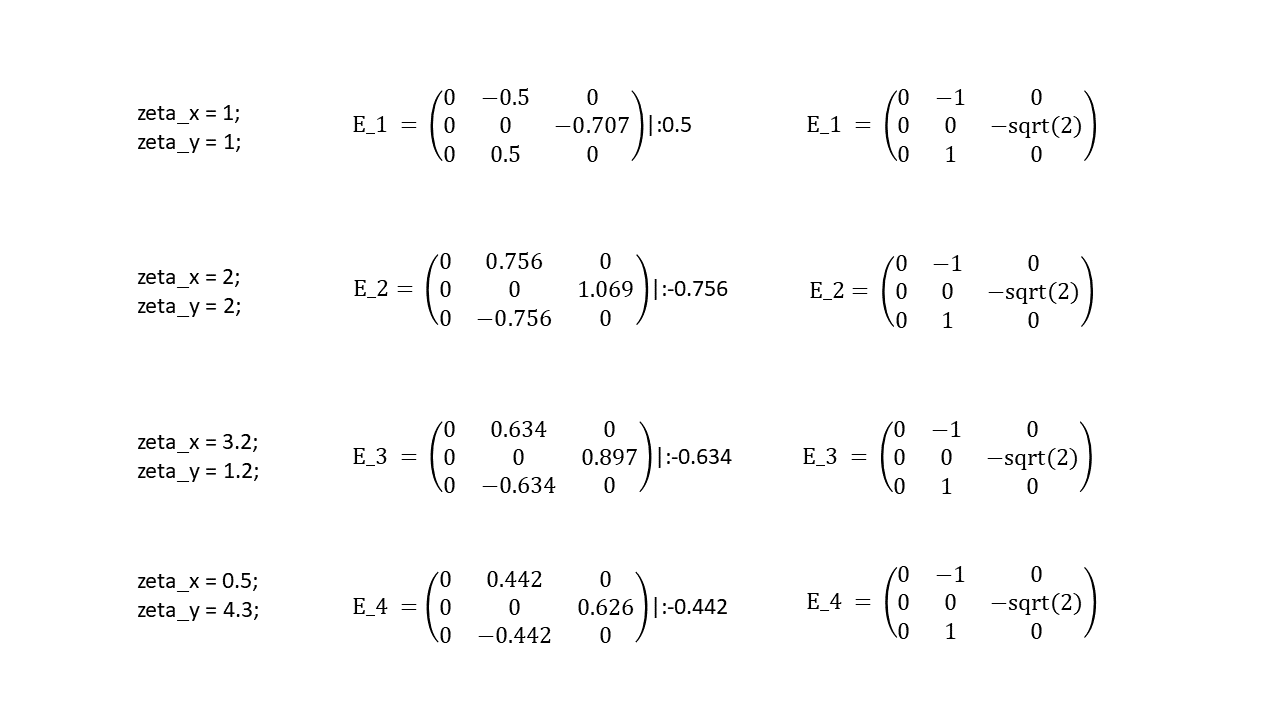
\includegraphics[width=1.\linewidth]{images/EMatrizen.png}
%	\captionof{figure}{Die essentiellen Matrizen sind bei jeder Auflösung, die gewählt wurden immer Vielfache voneinander} 
%\end{minipage}\\ \\

%Bei der Rekonstruktion der externen Kamerparameter ergibt sich daraus stehts die selbe Matrix für $P'$. Was wie gezeigt daran liegt, dass sich geometrisch nichts ändert, sondern lediglich die skalierung der Koordinatenwerte der Bildpunkte und somit auch eine Skalierung der Einträge in $F$ und $E$, welche aber ebenfalls als Skaleninvariant definiert sind\cite{HZ}. Die Ergebnisse der darauffolgenden Szenenrekonstruktionen, der einzelnen Szenen zeigt, dass sich immer die selbe Szene ergibt, welche mit der eigens aufgebauten Szene übereinstimmen.\\


\begin{minipage}{\linewidth}
	\centering
	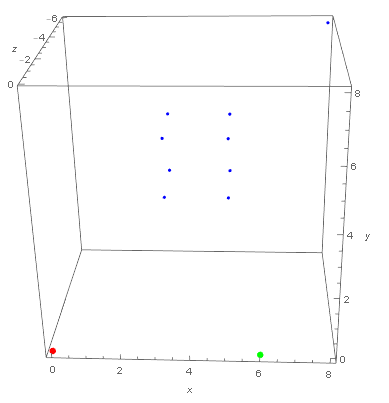
\includegraphics[width=0.5\linewidth]{images/DifferentAufloesungRekonstructedScene.png}
	\captionof{figure}{Die Abbildung zeigt die rekonstruierte Szenen des synthetischen Beispiels mit $K'_3$ als intrisische Parameter für $C'$.} 
	\label{fig: reconstructedDifferentResolutions}
\end{minipage}\\ \\

%Die Behauptung, dass die Auflösung der Kamera bei dem in dieser Arbeit gewählten Workflow für die Rekonstruktion der Szene keine Auswirkung hat, kann für das Minimalbeispiel bestätigt werden. \\

% zuerst Koordinatensysteme, was ändert sich ... Längenskalierung der Sensorkoordinatenachsen, da sich die Pixelskalierungen ändern.


 
% Hat als auswirkung: dass sich die Pixelwerte der Brennweiten ändern, jedoch nicht die Brennweite selbst 
% 
% Beispiel einbauen: Formel erweiterte Kameramatritze was ändert sich zeigen. 
% 
% Danach was ändert sich epipolargeoemtrisch für die rekonstruktion.
% 
% Der Punkt bleibt epipolargeometrisch der selbe... das dreieck ändert sich nicht.
% 
% Für die essentielle matrxc ändert sich nichts, da die kamermatrizen rausgezogen werden...hier formeln schreiben

%ob eine Änderung der Bildauflösung auch eine Änderung in den epipolargeometrischen Beziehungen, wie sie in Kapitel \ref{sec:HFE} hergeleitet wurden, mit sich bringt. 





%Für das Dreieck $	(\vec{C'}_\delta - \vec{C}_\delta) = (\vec{M}_\delta - \vec{C}_\delta) - (\vec{M}_\delta - \vec{C'}_\delta)$ zwischen den Projektionszentren und dem Objektpunkt bleibt unverändert. Im folgenden werden $F$ und $E$ aus den Gleichungen \ref{eq:Ep6} und \ref{eq:Ep7} aus Kapitel \ref{sec:EpiolarContraints} einmal mit gleichen Kameramatrizen $K =K'$ berechnet und einmal mit unterschiedlichen $K \neq K'$. 

%\begin{gather*}
%	F = K'^{-T}R'\left[ \vec{C'_\delta}-\vec{C_\delta}\right]_\times R^TK^{-1}\\
%	K = \begin{bmatrix}
%		1&0&0\\
%		0&1&0\\
%		0&0&1
%	\end{bmatrix} \;\;\;
%	K' = \begin{bmatrix}
%	2&0&0\\
%	0&3&0\\
%	0&0&1
%\end{bmatrix}\\
%R = \begin{bmatrix}
%	1&0&0\\
%	0&1&0\\
%	0&0&1\\ 
%\end{bmatrix}\;\;\;
%R'=\begin{bmatrix}
%	r&0&-r\\
%	0&1&0\\
%	r&0&r\\ 
%\end{bmatrix}\\
%	\left[ \vec{C'_\delta}-\vec{C_\delta}\right]_\times=
%	\begin{bmatrix}0&-(C'_{z\delta}-C_{z\delta})&C'_{y\delta}-C_{y\delta}\\
%		C'_{z\delta}-C_{z\delta}&0&-(C'_{x\delta}-C_{x\delta})\\
%		-(C'_{y\delta}-C_{y\delta})&C'_{x \delta}-C_{x\delta}&0\\
%	\end{bmatrix}\\
%	F = \begin{bmatrix}
%		2&0&0\\
%		0&3&0\\
%		0&0&1
%	\end{bmatrix}^{-T} 
%	\begin{bmatrix}
%		a&0&-a\\
%		0&1&0\\
%		a&0&a\\ 
%	\end{bmatrix}
%		\begin{bmatrix}0&-(C'_{z\delta}-C_{z\delta})&C'_{y\delta}-C_{y\delta}\\
%		C'_{z\delta}-C_{z\delta}&0&-(C'_{x\delta}-C_{x\delta})\\
%		-(C'_{y\delta}-C_{y\delta})&C'_{x \delta}-C_{x\delta}&0\\
%	\end{bmatrix} 
%	\begin{bmatrix}
%		1&0&0\\
%		0&1&0\\
%		0&0&1\\ 
%	\end{bmatrix}^T 
%	\begin{bmatrix}
%		1&0&0\\
%		0&1&0\\
%		0&0&1
%	\end{bmatrix}^{-1}\\
%F = \begin{bmatrix}
%	\frac{1}{2}&0&0\\
%	0&\frac{1}{3}&0\\
%	0&0&1
%\end{bmatrix}
%\begin{bmatrix}
%	r&0&-r\\
%	0&1&0\\
%	r&0&r\\ 
%\end{bmatrix}
%\begin{bmatrix}0&-(C'_{z\delta}-C_{z\delta})&C'_{y\delta}-C_{y\delta}\\
%	C'_{z\delta}-C_{z\delta}&0&-(C'_{x\delta}-C_{x\delta})\\
%	-(C'_{y\delta}-C_{y\delta})&C'_{x \delta}-C_{x\delta}&0\\
%\end{bmatrix} \\
%F= \begin{bmatrix}
%	\frac{1}{2}&0&0\\
%	0&\frac{1}{3}&0\\
%	0&0&1
%\end{bmatrix}
%\begin{bmatrix}
%	(C'_{z\delta}-C_{z\delta})r&0&(C'_{z\delta}-C_{z\delta})r\\
%	(C'_{z\delta}-C_{z\delta})&0&-(C'_{z\delta}-C_{z\delta})\\
%	-(C'_{z\delta}-C_{z\delta})r&0&(C'_{z\delta}-C_{z\delta})r
%\end{bmatrix}\\
%F=\begin{bmatrix}
%	\frac{1}{2}(C'_{z\delta}-C_{z\delta})r&0&\frac{1}{2}(C'_{z\delta}-C_{z\delta})r\\
%	\frac{1}{3}(C'_{z\delta}-C_{z\delta})r&0&-\frac{1}{3}(C'_{z\delta}-C_{z\delta})r\\
%		-(C'_{z\delta}-C_{z\delta})r&0&(C'_{z\delta}-C_{z\delta})r
%\end{bmatrix}
%\end{gather*}

%Berchnung Für F und E mit unterschiedlichen Auflösungen, was verändert sich für F  ?  E erklären, dass dadurch das K auf die Punkte berechnet wird E unverändert bleibt
%
%
%Jetzt noch irgendwie drauf verweisen dass bei der herleitung eh von K und K' ausgegangen wird also zwei unterschieldlichen Kameramatrizen....

%Für die Fundamentalmatrix und die essentielle Matrix ergeben sich verglichen mit denen aus dem ersten Beispiel mit Kameras gleicher Abbildung folgende Matrizen.\\





%\begin{gather}
%\vec{m_\sigma}=\begin{bmatrix}u \\v\\1 \end{bmatrix}=
%\begin{bmatrix}
%k_x&0&V_{\sigma,x}\\
%0&k_y&V_{\sigma,y}\\
%0&0&1&\\
%\end{bmatrix}
%\begin{bmatrix}m_{x \tau}\\ m_{y \tau}\\ 1\end{bmatrix}= R_\sigma \vec{m_\tau}\\
%\end{gather}
%
%Ändert sich die Auflösung so ändert sich $k_x$ und $k_y$, $V_{\sigma,x}$ und $V_{\sigma,y}$, da sich die Länge $l_x$ und die Breite $l_y$ verändern. Die Bildpunkte werden kann mit $k_x' = \frac{1}{l_x}'$ und $k_y' = \frac{1}{l_y}'$ skaliert. Die Translation des Hauptpunktes mit  $V_{\sigma,x}$ und $V_{\sigma,y}$ wird auch auf die neuen Sensorkoordinaten skaliert.
%
%\begin{gather}
%\vec{m_\sigma}'=\begin{bmatrix}u' \\v'\\1 \end{bmatrix}=
%\begin{bmatrix}
%k_x'&0&V_{\sigma,x}'\\
%0&k_y'&V_{\sigma,y}'\\
%0&0&1&\\
%\end{bmatrix}
%\begin{bmatrix}m_{x \tau}\\ m_{y \tau}\\ 1\end{bmatrix}= R_\sigma \vec{m_\tau}\\
%\end{gather}
%
%
%Wie schließ ich hier ab???


%\section{Synthetisches Beispiel mit unterschiedlichen Kameraauflösungen}

%Um die Aufgestellte Theorie zu überprüfen, wurde im synthetischen Beispiel die Kameramatrix von einer der beiden Kameras modifiziert. Für $C$ wurde $\zeta_x = \zeta_y = \zeta$ definiert, so das für Kameramatrix $K$ gilt:
%
%\begin{gather}
%	K = \begin{bmatrix}
%	1&0&0&0\\
%	0&1&0&0\\
%	0&0&1&0\\
%	%0&0&1&0
%	\end{bmatrix}
%\end{gather}
%
%Für $C'$ wurden drei verschiedene Kamermatrizen $K'$ definiert. Die resultierenden Abbildungen des Quaders sind in den Abbildungen \ref{fig:K},\ref{fig:K1},\ref{fig:K2} und \ref{fig:K3} zu sehen.
%
%Während für die Kameramatrix von $C$ der Wert  $\zeta_x = \zeta_y = 1$ in der Kamermatrix $K$ ist, wird das $\zeta$ in $C'$ verändert, so dass drei verschiedene neue Kameramatrizen $K'_1, K'_2$ und $K'_3$ ergeben. 
%
%
%
%\begin{gather}
%K = \begin{bmatrix}
%1&0&0&0\\
%0&1&0&0\\
%0&0&1&0\\
%%0&0&1&0
%\end{bmatrix}\\
%K'_1 = \begin{bmatrix}
%2&0&0&0\\
%0&2&0&0\\
%0&0&1&0\\
%%0&0&1&0
%\end{bmatrix}\\
%K'_2 = \begin{bmatrix}
%3.2&0&0&0\\
%0&1.2&0&0\\
%0&0&1&0\\
%%0&0&1&0
%\end{bmatrix}\\
%K'_3 = \begin{bmatrix}
%0.5&0&0&0\\
%0&4.3&0&0\\
%0&0&1&0\\
%%0&0&1&0
%\end{bmatrix}
%\end{gather}\\
%
%
%\begin{figure}[!htb]
%	\minipage{0.48\textwidth}
%	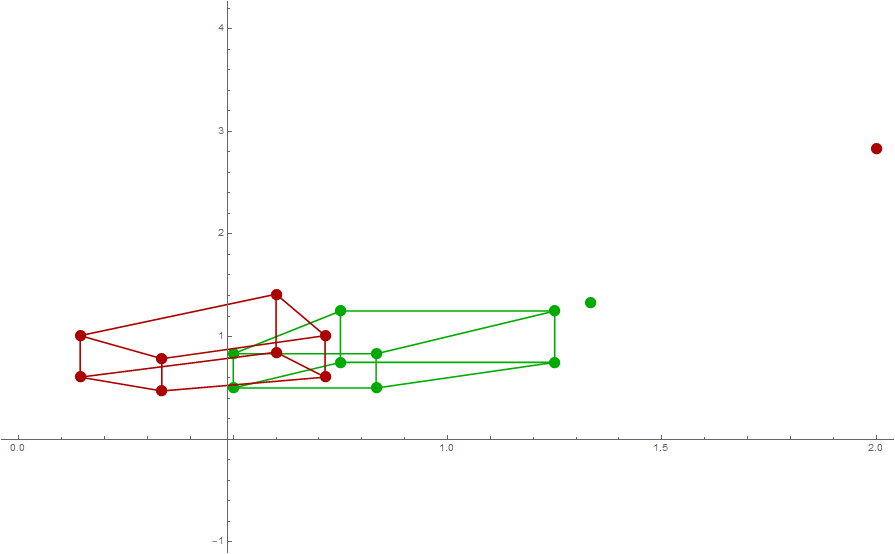
\includegraphics[width=\linewidth]{images/Zeta1.png}
%	\caption{$C$ und $C'$ haben die selbe Auflösung eingestellt}
%	\label{fig:K}
%	\endminipage\hfill
%	\minipage{0.48\textwidth}
%	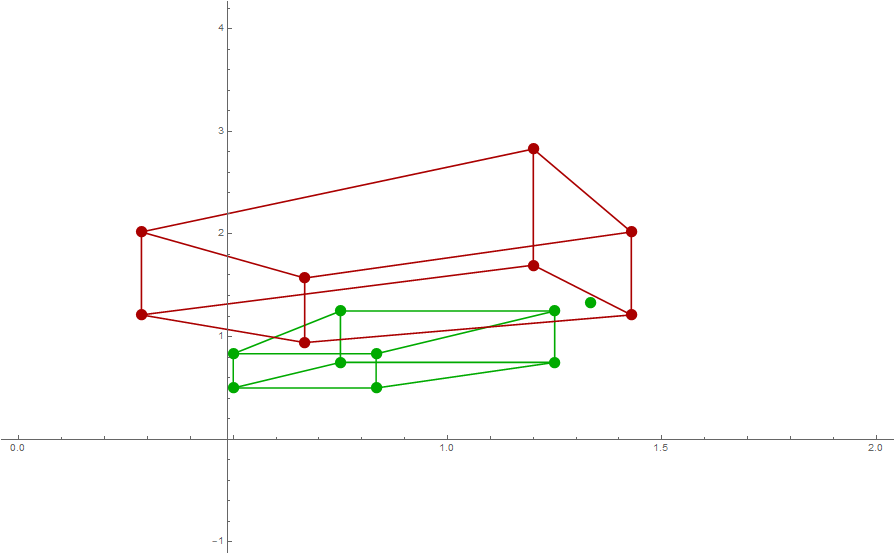
\includegraphics[width=\linewidth]{images/Zeta2.png}
%	\caption{$C$ und $C'$ haben unterschiedliche Auflösungen eingestellt. $C$ mit $K$ und $C'$ mit $K_1'$}
%	\label{fig:K1}
%	\endminipage\hfill
%\end{figure}
%
%\begin{figure}[!htb]
%	\minipage{0.48\textwidth}
%	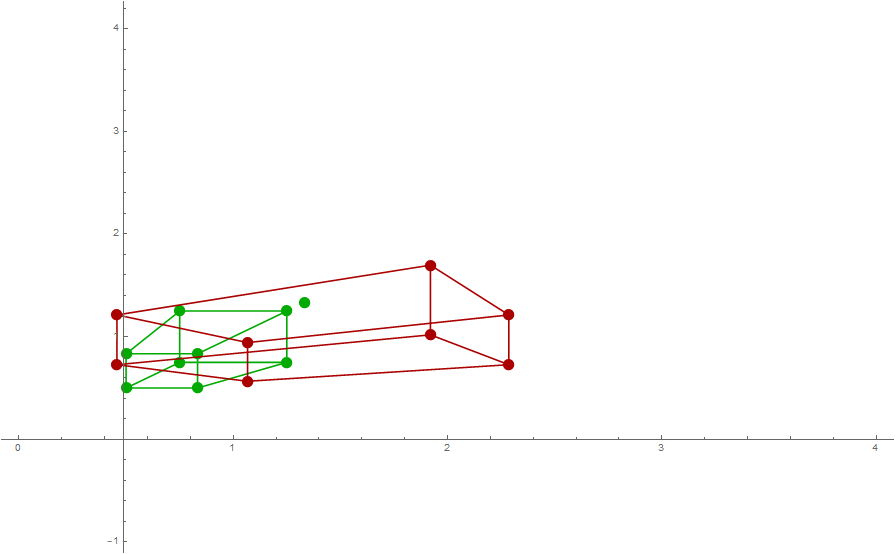
\includegraphics[width=\linewidth]{images/Zeta32_12.png}
%	\caption{$C$ mit $K$ und $C'$ mit $K_2'$}
%	\label{fig:K2}
%	\endminipage\hfill
%	\minipage{0.48\textwidth}
%	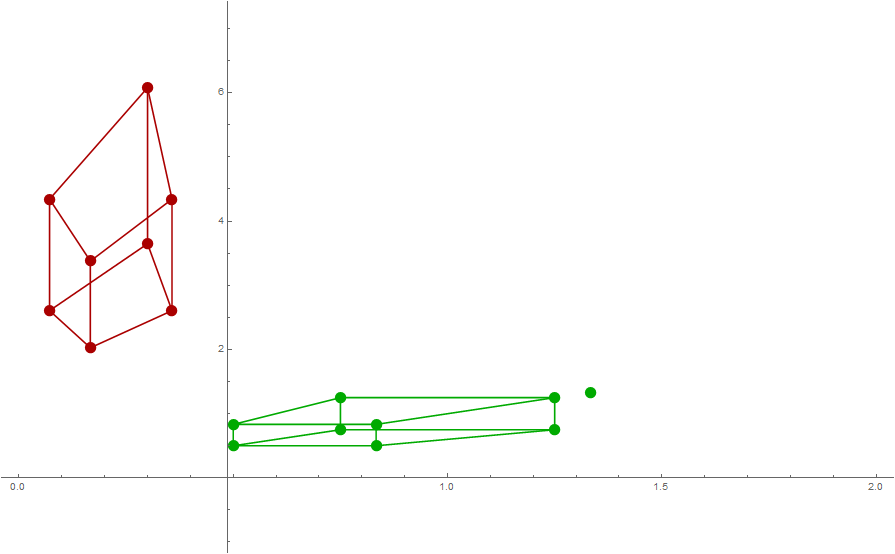
\includegraphics[width=\linewidth]{images/Zeta05_43.png}
%	\caption{$C$ mit $K$ und $C'$ mit $K_3'$}
%	\label{fig:K3}
%	\endminipage\hfill
%\end{figure}


%(GRAFIK $\zeta * 2, \zeta *3,2 und 1.2$, $\zeta * 0.5 und 4.3$ sagen dass das rote jeweils das mit dem verändertem $\zeta$ )\\

%
%Während die Abbildung von $C$ Unverändert bleibt, wird in Abbildung??? Die Abbildung des Quaders in $C'$ ''vergrößert'', was für eine höhere Anzahl an verwendeten Pixeln steht. In Abbildung ??? werden die Pixel in horizontaler Richtung um das 3.2- fache und in vertikaler Richtung um das 1.2-fache erweitert und in Abbilung ??? wird in horzontaler Richtung die Anzahl der Pixel um das 0.5-fache und in vertikaler Richtung um das 4.3-fache skaliert. 

%Für die essentielle Matrix ergeben sich verglichen mit denen aus dem ersten Beispiel mit Kameras gleicher Abbildung folgende Matrizen.\\


%\begin{gather*}
%	\zeta_x = 1, \, \zeta_y = 1: \; \; \;\;
%	F = \begin{pmatrix}
%			0&-0.5&0\\
%			0&0&\frac{1}{\sqrt{2}}\\
%			0&-0.5&0
%		\end{pmatrix} |: -0.5 \; \leadsto
%	F=\begin{pmatrix}
%		0&1&0\\
%		0&0&-\sqrt{2}\\
%		0&1&0
%	\end{pmatrix}\\	
%	\zeta_x = 2, \, \zeta_y = 2: \; \; \;
%	F = \begin{pmatrix}
%		0&0.378&0\\
%		0&0&-0.534\\
%		0&0.756&0
%	\end{pmatrix} |: 0.756 \; \leadsto
%	F=\begin{pmatrix}
%		0&0.5&0\\
%		0&0&-\frac{1}{\sqrt{2}}\\
%		0&1&0
%	\end{pmatrix}\\ \frac{1}{\zeta_x} = 0.5, \;\; \frac{\sqrt{2}}{\zeta_y} = \frac{1}{\sqrt{2}}\\
%	\zeta_x = 3.2, \, \zeta_y = 1.2: \; \; \;
%F = \begin{pmatrix}
%	0&0.198&0\\
%	0&0&-0.747\\
%	0&0.634&0
%\end{pmatrix} |: 0.634 \; \leadsto
%F=\begin{pmatrix}
%	0&0.312&0\\
%	0&0&-1.178\\
%	0&1&0
%\end{pmatrix}\\ \frac{1}{\zeta_x} = 0.312, \;\; \frac{\sqrt{2}}{\zeta_y} = -1.178\\
%	\zeta_x = 0.5, \, \zeta_y = 4.3: \; \; \;
%F = \begin{pmatrix}
%	0&0.885&0\\
%	0&0&-0.145\\
%	0&0.442&0
%\end{pmatrix} |: 0.442 \; \leadsto
%F=\begin{pmatrix}
%	0&2&0\\
%	0&0&-0.328\\
%	0&1&0
%\end{pmatrix}\\ \frac{1}{\zeta_x} =2, \;\; \frac{\sqrt{2}}{\zeta_y} = -0.328
%\end{gather*}\\

%\begin{minipage}{\linewidth}
%	\centering
%	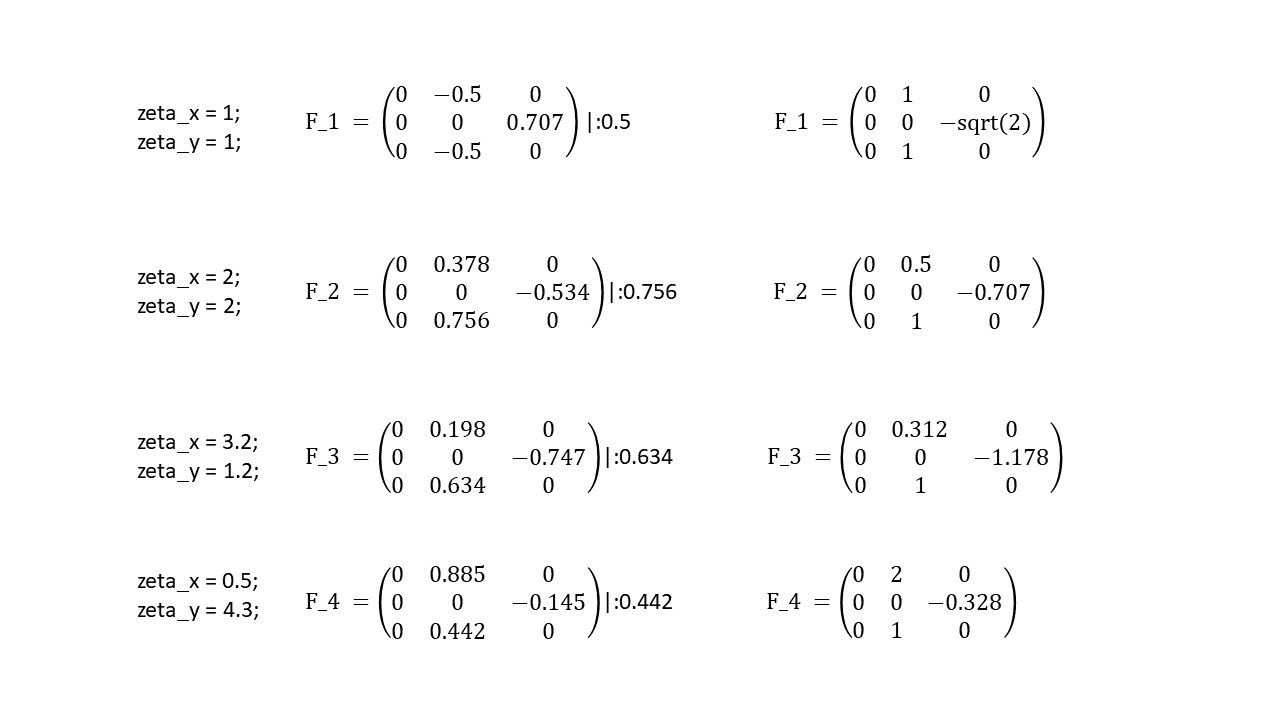
\includegraphics[width=1.\linewidth]{images/FundEMatrizen.png}
%	\captionof{figure}{Die Fundamentalmatrizen sind bei jeder Auflösung, die gewählt wurden immer Vielfache voneinander} 
%\end{minipage}\\ \\
%Die Werte für $\zeta_x$ wirken sich auf die erste Zeile der Fundamentalmatrix aus, während die Werte von $\zeta_y$ sich auf die zweite Zeile auswirken. Bei der nachfolgenden Umrechnung der Fundamentalmatrix in die essentielle Matrix mit Hilfe der Kameramatrizen $K$ und $K'$, kann festgestellt werden, dass die Ergebnisse jeweils Vielfache voneinander sind. \\


%(NICHT LÖSCHEN!DAS GEHÖRT ALLES IN KAPITEL 7!!!)
%Wenn man sich mit digitalen Bilddaten auseinandersetzt, so kommt man nicht drum herum sich auch mit den verschiedenen Auflösungsarten beschäftigen zu müssen.
%Aus der Stereokalibrierungsapp, welche \textit{MatLab} anbietet, ist bekannt, dass diese nicht mit Bildern unterschiedlicher Auflösung eine Szenerekonstruktion durchführen kann. 
%Der erste Schritt bestand erstmal darin zu überprüfen, warum zwei unterschiedliche Auflösungen in \textit{MatLab} Probleme machen. \textit{MatLab} verfolgt einen etwas anderen Rekonstruktionsansatz. Zu aller erst werden die Kameras kalibriert. Dies geschieht über die Matlab-Funktion \text{estimateCameraParameters}\cite{MatlabCamParam}. 
%Diese Funktion funktioniert auch bei Bildern unterschiedlicher Auflösung noch ohne Probleme. Das Problem, welches sich als eigentlich minimales Problem herausstellt, ist, dass die darauf folgenden Rektifizierung der Stereobilder nicht mit zwei Bildern unterschiedlicher Auflösung funktioniert. 
%In den \textit{MatLab} references, steht es nicht expliziet drin \cite{MatlabRec}. Die Rektifizierung in Matlab funktioniert nach einem Schema, welches ähnlich dem aufgezeigten Beispiel im Kapitel \nameref{sec:rectification} bereits erwähnt wurde und in \cite{Fusiello,FusielloSite} nochmal genau aufgeführt wird.
% Das Problem liegt also nicht daran, dass bilder unterschiedlicher Auflösung nicht rektifiziert werden können, sondern das Problem liegt an dem in \textit{MatLab} verwendeten Algorithmus für die Rektifizierung zweier Stereobilder (Foren Zitieren????). Warum \textit{MatLab} überhaupt rektifiziert, liegt daran, dass ein Ansatz der Szenerekonstruktion gewählt wurde, welcher die essentielle Matrix nicht benötigt. In diesem Falle, werden zwei Stereobilder aufgenommen, danach rektifiziert und anschließend über eine sogenannte \textit{Disparity-Map}, die Szenen punkte rekonstruiert\cite{MatlabDisp,MatlabStereoApp,Fusiello,Javier}. 
%Der in dieser Arbeit gewählte Rektifizierungsalgorithmus, ist nicht auf gleiche Kameraauflösungen beschränkt. Mittlerweile gibt es natürlich deutlich fortgeschrittenere Rektifizierungsansätze, jedoch wurde für diese Arbeit der Ansatz von \cite{ZZ} gewählt, um ein Gefühl zu vermitteln, dass wenn man sich auf die Epipolargeometrie bezieht, die Auflösungen der Kameras keine Rolle spielen\cite{Elements}.

